\documentclass[11pt,a4paper,twoside,openright,bachelor,english]{netthesis}
\usepackage[utf8]{inputenc}

% Include common packages
% raise package limit
\usepackage{etex}

% input encoding
\usepackage[utf8]{inputenc}

% subfiles
\usepackage{subfiles}
\makeatletter
\newif\ifsubfile\subfilefalse
\@ifclassloaded{subfiles}{\subfiletrue}{\subfilefalse}
\makeatother

% fonts
\usepackage[T1]{fontenc}
\usepackage{libertine}
\usepackage[scaled=0.8]{beramono}
\usepackage[expansion,protrusion,shrink=15,stretch=15]{microtype}
% Use libertine symbols --- Dirty hack!
% Does no longer work with new libertine package
%\DeclareTextCommand{\textbullet}{T1}{\libertineGlyph{bullet}}
%\DeclareTextCommand{\textdagger}{T1}{\libertineGlyph{dagger}}
%\DeclareTextCommand{\textdaggerdbl}{T1}{\libertineGlyph{daggerdbl}}
%\DeclareTextCommand{\textasteriskcentered}{T1}{\libertineGlyph{asteriskmath}}
% Alternatively use cmsy but get rid of warnings --- Dirty hack!
%\DeclareTextCommand{\textbullet}{T1}{$\bullet$}
%\DeclareTextCommand{\textdagger}{T1}{$\dagger$}
%\DeclareTextCommand{\textdaggerdbl}{T1}{$\ddagger$}
%\DeclareTextCommand{\textasteriskcentered}{T1}{$\ast$}

% vim: set sw=4 ts=4 et tw=0 :



% tables
\usepackage{array}
\usepackage{booktabs}
\usepackage{tabularx}
\usepackage{longtable}
\usepackage{ltxtable}

% lists etc
\usepackage{cite}

% text configurations not including font
%% define a long dash
\newcommand\drule{\rule[.56ex]{\widthof{-}}{.1ex}}
\newcommand\nrule{\rule[.56ex]{\widthof{--}}{.1ex}}
\newcommand\mrule{\rule[.56ex]{\widthof{---}}{.1ex}}
\newcommand\lrule{\rule[.56ex]{1em}{.1ex}}

% reset some length
\setlength{\textfloatsep}{1.7\baselineskip plus 0.6\baselineskip minus 0.4\baselineskip}

% vim: set sw=4 ts=4 et tw=0 :



% math
\usepackage{mathtools}
\usepackage{packages/accents}
\usepackage{fixmath} % upper case Greek letters in italics.
% All mathematical definitions
% use msvsymbols package
%\usepackage{msvsymbols}

\usepackage[libertine,cmintegrals,libaltvw]{newtxmath}
\usepackage[
bb=ams,
scr=rsfs,
cal=cm
]{mathalfa}

% libertine math font stuff
\makeatletter
\DeclareMathSymbol{0}\mathalpha{operators}{"30}
\DeclareMathSymbol{1}\mathalpha{operators}{"31}
\DeclareMathSymbol{2}\mathalpha{operators}{"32}
\DeclareMathSymbol{3}\mathalpha{operators}{"33}
\DeclareMathSymbol{4}\mathalpha{operators}{"34}
\DeclareMathSymbol{5}\mathalpha{operators}{"35}
\DeclareMathSymbol{6}\mathalpha{operators}{"36}
\DeclareMathSymbol{7}\mathalpha{operators}{"37}
\DeclareMathSymbol{8}\mathalpha{operators}{"38}
\DeclareMathSymbol{9}\mathalpha{operators}{"39}
\makeatother

%% math alphabet fonts
\DeclareSymbolFont{nxlmibit}{OML}{nxlmi}{bx}{it}
\DeclareSymbolFontAlphabet{\mathbit}{nxlmibit}
%FIMXE: the first package seems to cause an \if\fi bug
%\DeclareSymbolFont{libertineplus}{T1}{ntxrx}{m}{n}
%\DeclareMathSymbol{+}{\mathbin}{libertineplus}{43}

\newcommand\showmathalphabet{\noindent\begin{tabular}{ll}
    mathnormal  & $abcdefghijklmnopqrstuvwxyz$\\
                & $ABCDEFGHIJKLMNOPQRSTUVWXYZ$\\
    mathrm      & $\mathrm{abcdefghijklmnopqrstuvwxyz}$\\
                & $\mathrm{ABCDEFGHIJKLMNOPQRSTUVWXYZ}$\\
%    mathit      & $\mathit{abcdefghijklmnopqrstuvwxyz}$\\
%                & $\mathit{ABCDEFGHIJKLMNOPQRSTUVWXYZ}$\\
    mathbf      & $\mathbf{abcdefghijklmnopqrstuvwxyz}$\\
                & $\mathbf{ABCDEFGHIJKLMNOPQRSTUVWXYZ}$\\
    mathbit     & $\mathbit{abcdefghijklmnopqrstuvwxyz}$\\
                & $\mathbit{ABCDEFGHIJKLMNOPQRSTUVWXYZ}$\\
%    mathfrak    & $\mathfrak{abcdefghijklmnopqrstuvwxyz}$\\
%                & $\mathfrak{ABCDEFGHIJKLMNOPQRSTUVWXYZ}$\\
    mathcal     & $\mathcal{ABCDEFGHIJKLMNOPQRSTUVWXYZ}$\\
%    mathscr     & $\mathscr{ABCDEFGHIJKLMNOPQRSTUVWXYZ}$\\
%    matheus     & $\matheus{ABCDEFGHIJKLMNOPQRSTUVWXYZ}$\\
\end{tabular}}

% vim: set sw=4 ts=4 et tw=0 :



% theorems
%% theorems and proofs
\newtheoremstyle{reportitalic}%
    {2ex}{2ex}{\normalfont\renewcommand\em\upshape\itshape}{}%
    {\normalfont\scshape}{.}{1em}{}
\newtheoremstyle{reportnormal}%
    {2ex}{2ex}{\normalfont}{}%
    {\normalfont\scshape}{.}{1em}{}
\theoremstyle{reportitalic}
\newtheorem{definition}{Definition}[chapter]
\newtheorem{theorem}{Theorem}[chapter]
\newtheorem{proposition}[theorem]{Proposition}
\newtheorem{corollary}[theorem]{Corollary}
\newtheorem{lemma}[theorem]{Lemma}
\theoremstyle{reportnormal}
\newtheorem{example}{Example}[chapter]
\newtheorem{remark}{Remark}[chapter]

% theorem enumerates
\newenvironment{thmenum}{\begin{enumerate}
    \setlength\itemsep{.2ex}
    \setlength\parsep{0pt}
    \setlength\parskip{0pt}
    \renewcommand\theenumi{\alph{enumi}}
    \renewcommand\labelenumi{(\theenumi)}
    \vskip -\topsep\vskip .2ex\vskip 0pt
}{\end{enumerate}}

% proof reference of theorem enumerates
\newcommand\proofrefskip{\hskip 1em\relax}
\newcommand\proofref[1]{(\ref{#1})}

% vim: set sw=4 ts=4 et tw=0 :



% listings
\usepackage{listings}

% drawing and graphics
\usepackage{packages/tumcolors}
\usepackage{tikz}
\usetikzlibrary{calc,arrows,matrix,positioning,shapes.multipart,shapes.geometric}

% commutative diagram
\tikzstyle{commutative diagram}=[matrix of math nodes,
    matrix anchor=m-1-1.base,anchor=base,
    row sep=3em,column sep=4em,
    minimum width=3em,minimum height=2em]
\tikzstyle{commutative edge}=[]
\tikzstyle{map}=[commutative edge,->]
\tikzstyle{injective map}=[commutative edge,right hook->]
\tikzstyle{surjective map}=[commutative edge,->>]
\tikzstyle{bijective map}=[commutative edge,right hook->>]

% broadcast diagrams
\tikzstyle{wireless}=[draw,thick,circle,
    minimum size=5.5mm,inner sep=0mm,font=\small]
\tikzstyle{virtual}=[draw,thick,rectangle,
    minimum size=5.5mm,inner sep=0mm,font=\small]
\tikzstyle{arc}=[draw,thick,->]
\tikzstyle{rate}=[pos=.5,above,sloped,font=\small]
\tikzstyle{broadcast}=[draw,thin,dashed]
\tikzstyle{broadcast rate}=[font=\small]
\tikzstyle{cut}=[draw,thick]

% Markov chains
\newcommand\clamp[1]{\raisebox{0pt}[0pt][0pt]{\makebox[0pt][c]{#1}}}
\newcommand\clampwd[1]{\raisebox{0pt}[\height][0pt]{\makebox[0pt][c]{#1}}}
\newcommand\clamphd[1]{\raisebox{0pt}[0pt][0pt]{\makebox[\width][c]{#1}}}

% vim: set sw=4 ts=4 et tw=0 :


\usepackage{packages/moeptikz}

% IEEE tools for tweaking bib style
\usepackage{packages/IEEEtrantools}

% enable links
\usepackage[colorlinks=false,pdfborder={0 0 0}]{hyperref}
\newcommand\toc{\relax}

% pgfplots
\usepackage{pgfplots}
\pgfplotsset{compat=newest}
\pgfplotsset{colormap={moepcolormap}{[1cm] color(0cm)=(black!60) color(5cm)=(black!1)}}
%\pgfplotsset{colormap={moepcolormap}{[1cm] color(0cm)=(TUMDarkerBlue) color(1cm)=(TUMLighterBlue) color(2cm)=(TUMGreen) color(3cm)=(TUMBeamerYellow) color(4cm)=(TUMOrange) color(5cm)=(I8LogoRed)}}



% Maybe we want to inlcude some additional packages


% hyphenation
\hyphenation{op-ti-cal net-work net-works semi-con-duc-tor tech-nique tech-niques}


% Needed for Bachelor's theses, Master's theses and IDP
\titlegerman{Leistungsanalyse der Funktionen von Middleboxes}
\titleenglish{Performance analysis of Middlebox functionality}
\submitteddate{\today}
\author{Simon Sternsdorf}
\supervisor{\NEThead}
\advisor{Florian Wohlfart}

% Additionally needed for dissertations
\committeechair{}
\committeeexaminers{}{}{}
\accepteddate{}


\begin{document}%

% Makes sure that same author names are not replaced by dahes
\bstctlcite{IEEEexample:BSTcontrol}

\pagenumbering{gobble}
\maketitle%


\subfile{include/abstract.tex}


\pagenumbering{Roman}%

{\tableofcontents}
{\listoffigures}
{\listoftables}

\cleardoublepage

\pagenumbering{arabic}

\chapter{Introduction}

\section{Motivation}
Middleboxes are mediating devices used by both End-user Internet Service Providers and normal home users. The requirements ISPs have for Middleboxes are of course vastly different from the requirements of private users. Thus the implementations differs greatly as well. Middleboxes for home users do not have high performance requirements. They conduct mostly very simple tasks for a low amount of devices. This is changing of course, as more and more web-enabled devices are used in modern households. 
Still the required performance is low in contrast to at an ISP for example. Especially carrier grade network address translation is used to provide ipv4 connectivity for mobile phones, since IPv4 addresses are getting rare \cite{A10}. The middleboxes used are mostly implemented in hardware, which has assets and drawbacks. Those drawbacks are significant. 
Middleboxes specifically produced for ISPs are expensiv both in acquisition and maintainance, also they usually have to be replaced to introduce new features \cite{WhiteP}. Also they are difficult to scale with higher or lower demand. All these problems are avoidable through network function virtualization. And the long-term plan is indeed to replace these hardware middleboxes with all-purpose hardware that is cheap and easily replaceable \cite{Click}. The networking functions would be implemented in software. 7 of the worlds largest telecoms network operators are in an standards group for virtualization of network functions. So the topic is already being discussed in ISPs \cite{NetDis} 



\section{Goal of the thesis}
The goal of this thesis is to test different software Middlebox implementations. We will install different middlebox implementations in our testbed. Then we will test the packet processing capability, try to find bottlenecks for the performance when processing packets. We will evaluate our results. 
Additionally we want to evaluate if software Middleboxes are competitive with hardware implemented Middleboxes and could replace them in the foreseeable future. 
ection{Outline}

The thesis reads as follows. The second chapter introduces the theoretical concept of NAT and a NAT model which we used in our tests. Also it defines performance testing. Additionally the Data Plane Development Kit is introduced, DPDK. The third chapter informs the reader about the general idea behind our tests. Further it presents the software used for the tests. This includes the software running on the device under test, as well as the software used to run the tests. It explains the methodological approach used in this thesis. Here it explains the setup for the experiment. In chapter 4 are the collected results of the Firewall and NAT tests with a brief analysis of the result. Finally chapter 5 summarizes the outcome and gives possible future works of this thesis. 

\chapter{Background}

This chapter gives a overview over network address translation and the NAT model we will assume in this thesis. Also it will explain our approach to performance testing. Finally the chapter outlines the Data Plane Development Kit, developed by Intel \cite{DPDKOv}.

\section{NAT}

Network address translation NAT was first described 1993 and written into \href{https://tools.ietf.org/html/rfc3022.html}{RFC 3022} in 2001. It was proposed as an temporary solution for the shortage of IPv4 addresses. It should slow down the need for IPv4 addresses of private customers and businesses \cite{bonaventure2011computer}. It does this by working as a connector between 2 different networks with different IPv4 address spaces. Mostly it translates between the address space of the internet and a private network. Since NAT is used so broadly it is one of the most common middleboxes. $\newline$
NAT in private households is in many instances implemented directly in the router. The home ususally only gets one IPv4 address from its ISP. The router then interconnects the home network to the internet via an ISP. It translates the private IP addresses of the home network to enable them to share the single IPv4 address \cite{bonaventure2011computer}[Page 168]. In corporate networks it basically fulfills the same purpose. The main difference is that the border router manages multiple public IPv4 addresses and manages the correct translation between them and the private IPv4 addresses in the private network. 
Here we see the simple version with only one public IPv4 address.

\begin{figure}[h]
\centering
{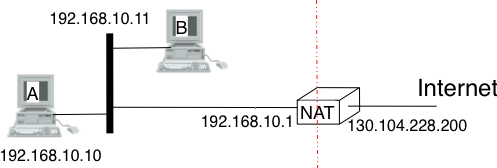
\includegraphics[width=.75\columnwidth]{figures/NATPrivate}} \quad
\caption[A simple NAT with one public IPv4 address]{ A simple NAT with one public IPv4 address \cite{bonaventure2011computer}[Page 168]}
\label{fig:NATPrivate}
\end{figure}

A NAT middlebox manages the translation between the different IPv4 address spaces. To achieve this the middlebox has to save a mapping of the private IP addresses to the public ones. In the simplest imaginable case we have as many public IPv4 addresses as we have private ones. In that case the mapping is simply a bijection. When the NAT middlebox receives a packet from a new private IP S in the internal network it maps it to a not used public IP from its address pool. This mapping is saved. To translate the packet the NAT middlebox has to : $\newline$
\begin{enumerate}

\item Replace the original source IP from the packet with the mapped public IP
\item Completely recompute the IP header checksum, as not only the Time To Live header field changes, but also the source IP header field \cite{tanenbaum1996computer}[Page 435]
\item Recompute the checksum in the TCP or UDP header if existent. The checksum of these protocols computes the checksum over the whole packet

\end{enumerate} 

When an answer from the internet arrives the NAT middlebox has to to the same process only with replacing the destination IP address with the source address of the private host. This is done with the same mapping. Afterwards the packet is forwarded to the host in the private network. $\newline$
In the realistic case where we have less public IP addresses then private ones the translation occurs over the IP and the port number. An NAT middlebox that uses this translation method maps the internal IP and the internally used port number of the TCP or UDP packet to a public IP from the IP pool available to the NAT middlebox and the first available port number \cite{bonaventure2011computer}[Page 169]. The entries in the mapping table are removed by the system after either the TCP connection is closed or the connection is idle for a longer time. Here the NAT middlebox functions similarly to a stateful firewall, which will become important later. 
When the NAT middlebox has to handle packets from the internet, it looks up a mapping from its state table for the destination IP address and the destination port. If a matching mapping exists the packet is translated accordingly and forwarded to the matching internal host. If no such mapping exists the packet gets discarded, as there is no way to determine the correct internal host. $\newline$
NAT has two main disadvantages: Opening TCP connections from the internet to an internal network is very difficult. This means that for example FTP users behind NAT have problems. In active mode, the FTP client first establishes a control connection to the server.After that the client listens on a random port for the incoming data connection from the server. If the client sits behind a NAT this connection will not work \cite{FTP}.$\newline$
The other disadvantage is that NAT breaks the end- to end transparency of the IP layer and the application layer. This problem occurs when the IP address is used in the application layer, as the NAT only replaces the IP in the IP header. This can be avoided with an Application Level Gateway installed at the NAT. However it is not feasible to install an an ALG for every application that relies on the IP in layer 7. 

\section{NAT model}

\section{Performance testing}

\section{Data Plane Development Kit}

\chapter{Methodology}

\section{General Idea}

\subsection{Software}

\section{Test Methodology}

\subsection{Experimental Setup}

\subsection{MoonGen Traffic Generator}

\subsection{Open VSwitch}

\subsection{mOS}

\chapter{Evaluation and Analysis of results}

\section{Firewall tests}

\section{NAT tests}

\chapter{Conclusion}

\section{Future Works}


%\subfile{include/outline.tex}
\appendix
%\subfile{Appendix.chap.tex}

%\subfile{Nomenclature.chap.tex}



\bibliographystyle{packages/IEEEtran}
\bibliography{lit}

\end{document}

% vim: set sw=4 ts=4 et tw=72 :

